\documentclass[a4paper,12pt]{article}
\usepackage[a4paper, margin=2.5cm]{geometry}
\usepackage[pdftex]{graphicx}
\usepackage{tikz}
\usepackage{pgfplots}
\usepackage{enumitem}
\usepackage{float}
\usepackage[document]{ragged2e}
\usepackage[utf8]{inputenc}
\usepackage[T1]{fontenc}
\usepackage[spanish,es-tabla]{babel}
\renewcommand{\shorthandsspanish}{}
\usepackage{xurl}
\usepackage{lipsum}
\usepackage{mwe}
\usepackage{multicol}
\usepackage{siunitx}
\usepackage{listings}
\usepackage{enumitem}
\usepackage{amsmath}
\usepackage{listings}

\graphicspath{ {/home/saikkopat/Documents/school/DB/P2/} }

\begin{document}

\begin{titlepage}
	\begin{tikzpicture}[overlay, remember picture]
		\path (current page.north east) ++(-0.3,-1.5) node[below left] {
\includegraphics[width=0.35\textwidth]{/home/saikkopat/Documents/LOGOS IPN/EscudoESCOM}};
	\end{tikzpicture}
	\begin{tikzpicture}[overlay, remember picture]
		\path (current page.north west) ++(1.5,-1) node[below right] {
\includegraphics[width=0.2\textwidth]{/home/saikkopat/Documents/LOGOS IPN/logo}};
	\end{tikzpicture}
	\begin{center}
		\vspace{-1.5cm}
		{\LARGE Instituto Politécnico Nacional\par}
		\vspace{.5cm}
		{\LARGE Escuela Superior de Cómputo\par}
		\vspace{2.5cm}
		{\large Unidad de aprendizaje:}\\{\Large Bases de datos\par}
		\vspace{7cm}
		{\scshape\Huge Práctica 2:\par}
		{\itshape\Large Introducción a PostgreSQL\par}
		\vfill
		{\Large Alumno: González Cárdenas Ángel Aquilez\par}
		\vspace{1cm}
		{\Large Boleta: 2016630152\par}
		\vspace{1cm}
		{\Large Grupo: 3CV1\par}
		\vspace{1cm}
		{\Large Profesor: Blanco Almazán Iván Eduardo\par}
		\vfill
	\end{center}
\end{titlepage} 

\newpage

\section{Objetivos}

\begin{enumerate}
	\item Instalar de forma adecuada el sistema gestor de base de datos \emph{PostgreSQL}.
	\item Crear una base de datos que contenga una tabla y registros.
\end{enumerate}

\section{Introducción}

El sistema gestor de bases de datos que ahora conocemos como \emph{PostgreSQL} tiene sus origenes en el proyecto \emph{POSTGRES}, creados en la Universidad de California en Berkeley.\\

Para poder trabajar con \emph{PostgreSQL}, primero se instaló el software en el sistema operativo GNU/Linux \emph{Xubuntu}, nombre compuesto de el sistema operativo base Ubuntu y el entorno de escritorio XFCE.\\

Ejecutamos el siguiente comando en la terminal:\\

\begin{lstlisting}
sudo apt install postgresql
\end{lstlisting}


Una vez terminada la instalación, procedemos a verificar el estatus del \emph{daemon} con el siguiente comando:\\

\begin{lstlisting}
service postgresql status
\end{lstlisting}

el cual nos devuelve la siguiente información:\\

\vspace{.5cm}

\begin{figure}[!h]
\centering
	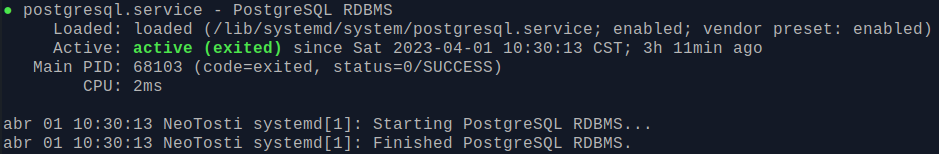
\includegraphics[width=.7\textwidth]{fig1}
	\label{fig1}
	 \caption{Estatus del \emph{daemon}}
\end{figure}


\vspace{.5cm}

Finalmente ingresamos a la linea de comandos introduciendo lo siguiente:

\begin{lstlisting}
sudo -u postgres psql
\end{lstlisting}


Una vez dentro, verificamos el estado de la conexión mediante el comando \textbackslash conninfo que en conjunto, nos arrojaron lo siguiente:\\


\begin{figure}[!h]
\centering
	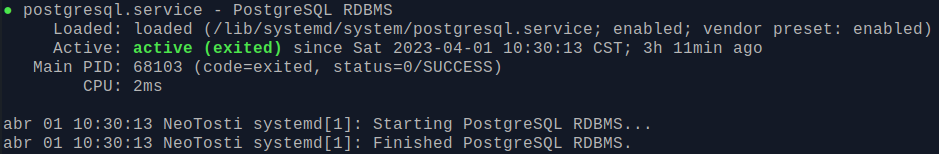
\includegraphics[width=.7\textwidth]{fig1}
	\label{fig2}
	 \caption{Ingreso a la linea de comandos de \emph{PostgreSQL}}
\end{figure}


\section{Desarrollo}

\subsection{Creación de la base de datos}

Comenzamos creando una base de datos simple, la cual denominamos \texttt{springfield} mediante el siguiente comando de SQL:

\begin{lstlisting}
CREATE DATABASE SPRINGFIELD;
\end{lstlisting}

Después comprobamos su existencia con el comando \textbackslash l:

\begin{figure}[!h]
\centering
	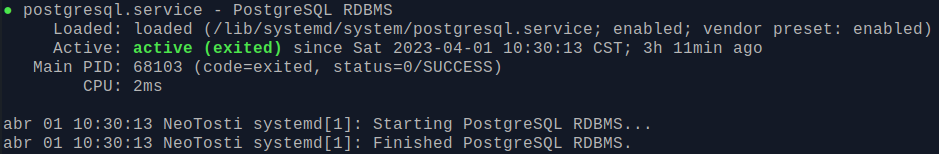
\includegraphics[width=.7\textwidth]{fig1}
	\label{fig3}
	 \caption{Listado de todas las bases de datos disponibles}
\end{figure}

Ingresamos a nuestra base de datos con el comando \textbackslash c seguido del nombre, en este caso:

\begin{lstlisting}
	\c 	springfield
\end{lstlisting}

y nos arrojó el siguiente mensaje:\\

\begin{figure}[!h]
\centering
	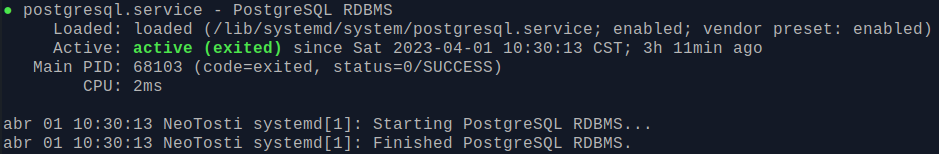
\includegraphics[width=.7\textwidth]{fig1}
	\label{fig4}
	 \caption{Conexión exitosa a la base de datos}
\end{figure}

\subsection{Creación de una tabla y elementos}

Dentro de la base de datos, creamos la tabla \texttt{persona}, que contiene los siguientes campos:\\

\begin{enumerate}
	\item id \texttt{SERIAL PRIMARY KEY},
	\item nombres \texttt{VARCHAR},
	\item ap\_paterno \texttt{VARCHAR},
	\item ap\_materno \texttt{VARCHAR},
	\item fecha\_nacimiento \texttt{DATE},
	\item sexo \texttt{CHAR}
\end{enumerate}

Con el comando CREATE TABLE y nuestros atributos definidos, ingresamos:\\

\begin{lstlisting}[language=sql]
CREATE TABLE PERSONA (
	id SERIAL PRIMARY KEY,
	nombres VARCHAR,
	ap_paterno VARCHAR,
	ap_materno VARCHAR,
	fecha_nacimiento DATE,
	sexo CHAR
);
\end{lstlisting}

Y con el comando \textbackslash d seguido del nombre de la tabla, comprobamos que se creo de manera adecuada:

\begin{figure}[!h]
\centering
	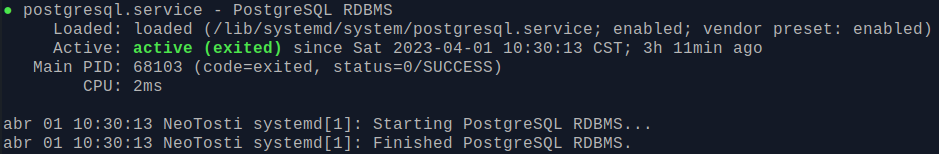
\includegraphics[width=.7\textwidth]{fig1}
	\label{fig5}
	 \caption{Creación de la tabla personas}
\end{figure}

Luego, agregamos los siguientes registros:\\

\begin{lstlisting}[language=sql]
INSERT INTO PERSONA VALUES
		(1,'Homero','Simpson','J','12-05-1956','M');
INSERT INTO PERSONA VALUES
		(2,'Marge','Simpson', 'Bouvier','19-03-1956','F');
\end{lstlisting}

y para comprobar su existencia, se consultan mediante la sentencia:

\begin{lstlisting}
SELECT * FROM PERSONA;
\end{lstlisting}

produciendo así el siguiente resultado:\\

\begin{figure}[!h]
\centering
	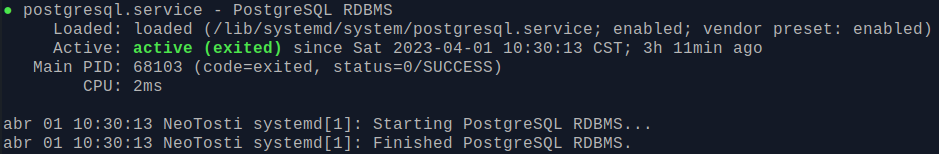
\includegraphics[width=.7\textwidth]{fig1}
	\label{fig6}
	 \caption{Registros en la tabla \texttt{persona}}
\end{figure}

\newpage

\section{Conclusión}

Al termino de la práctica, se instaló el sistema gestor de base de datos PostgreSQL, se creo una base de datos con una tabla y se ingresaron registros, permitiendo así cumplir con los objetivos planteados.\\

\section{Referencias}

\begin{itemize}
\item A Brief History of PostgreSQL. (2023, febrero 9). PostgreSQL Documentation.\\https://www.postgresql.org/docs/current/history.html

\item Levinas, M. (s/f). How to Install and Setup PostgreSQL server on Ubuntu 20.04. Cherry Servers. Recuperado el 1 de abril de 2023, de\\https://www.cherryservers.com/blog/how-to-install-and-setup-postgresql-server-on-ubuntu-20-04
\end{itemize}


\end{document}